\documentclass[12pt,titlepage]{article}
\usepackage[margin=1.25in]{geometry}
\usepackage{fancyhdr,tabularx,graphicx,tikz,longtable,tabu,amsmath}
\usetikzlibrary{svg.path,calc}
\tikzstyle{square} = [rectangle, draw, text centered, minimum height=2em, minimum width=5cm]
\tikzstyle{arrow} = [line width=0.5mm,->]

\usepackage{minted}
\definecolor{bg}{rgb}{0.08,0.09,0.12}
\definecolor{lightBg}{rgb}{0.8,0.8,0.8}
\usemintedstyle{github-dark}

\pagestyle{fancy}
\setlength{\headheight}{15pt} % compensate fancyhdr style
\fancyhead{}
\fancyfoot{}
\fancyfoot[L]{\thepage}
\fancyfoot[R]{\textit{Basic Programming Practicum - Jobsheet 3 Experiment}}
\renewcommand{\footrulewidth}{0.4pt}% default is 0pt, overline for footer

\newcommand{\details}[2]{
#1 & #2  \\
}

\begin{document}
\begin{titlepage}
    \centering
    \vfill
    {\bfseries\LARGE
        Basic Programming Practicum\\
        \vskip0.25cm
        Jobsheet 3 Experiment
    }
    \vfill
    
\includegraphics[width=6cm]{images/polinema-logo.png}
    \vfill
    {\textbf{Name}\\
        Dicha Zelianivan Arkana\\
        \vskip0.5cm
        \textbf{NIM}\\
        2241720002\\
        \vskip0.5cm
        \textbf{Class}\\
        1i\\
        \vskip0.5cm
        \textbf{Department}\\
        Information Technology\\
        \vskip0.5cm
        \textbf{Study Program}\\
        D-IV Informatics Engineering}
\end{titlepage}

\section{Practice}
\subsection{Experiment 1}
\begin{enumerate}
    \item Open a text editor
    \item Create a new file, give it a name \texttt{\textbf{ExampleVariable.java}}
    \item Write the basic structure of the Java programming language which contains the \texttt{main()} function.
    \item { 
        Write the code below inside the \texttt{public static void main(String[] args)}
        
        \begin{figure}[h]
            \centering
            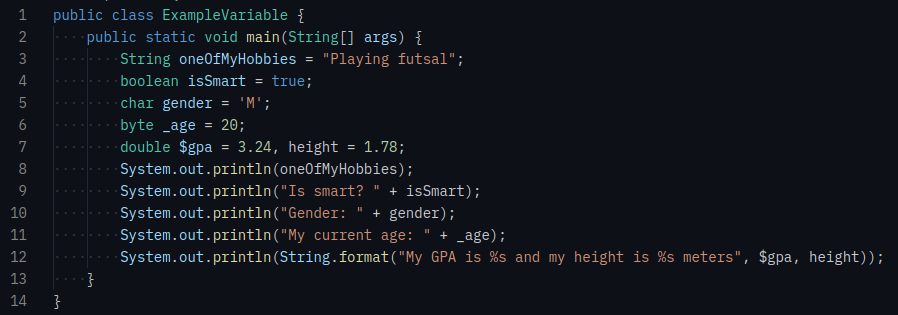
\includegraphics[width=0.9\textwidth]{./images/variable-code.png}
            \caption{The code for Experiment 1}
        \end{figure}
        \begin{figure}[h]
            \centering
            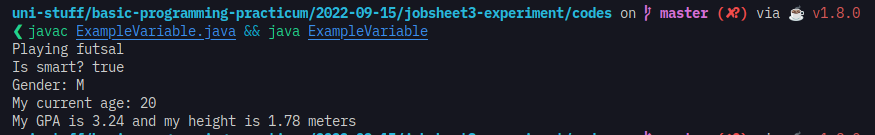
\includegraphics[width=0.9\textwidth]{./images/variable-output.png}
            \caption{The output for Experiment 1}
        \end{figure}
    }
\end{enumerate}
\pagebreak
\textbf{Questions}
\begin{enumerate}
    \item { 
        Change the variable name so that it look better and more correct!

        \begin{figure}[h]
            \centering
            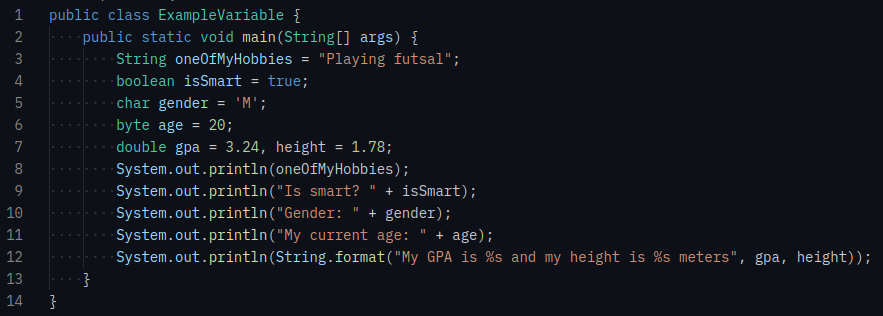
\includegraphics[width=0.9\textwidth]{./images/variable-code-updated.png}
            \caption{The code for Experiment 2}
        \end{figure}
    }
\end{enumerate}

\subsection{Experiment 2}
\begin{enumerate}
    \item Open a text editor
    \item Create a new file, give it a name \texttt{\textbf{ExampleDataType.java}}
    \item Write the basic structure of the Java programming language which contains the \texttt{main()} function.
    \item {
        Write the code below inside the \texttt{public static void main(String[] args)}
        
        \begin{figure}[h]
            \centering
            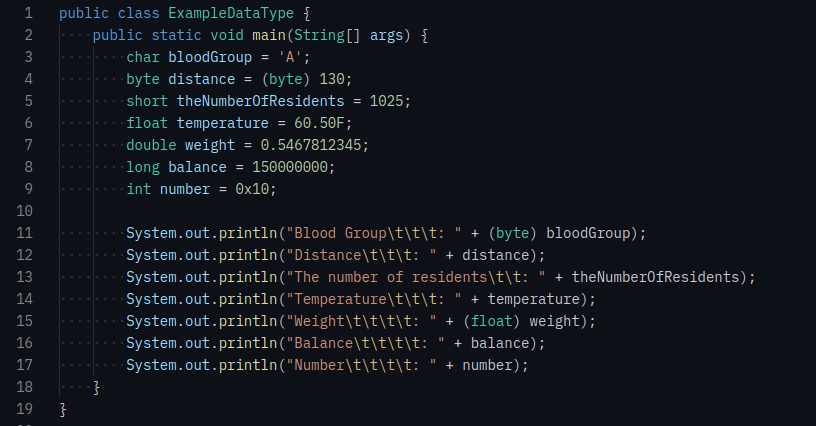
\includegraphics[width=0.8\textwidth]{./images/datatype-code.png}
            \caption{The code for Experiment 2}
        \end{figure}
    }
    \pagebreak
    \item {
        Execute the program and observe the result

        \begin{figure}[h]
            \centering
            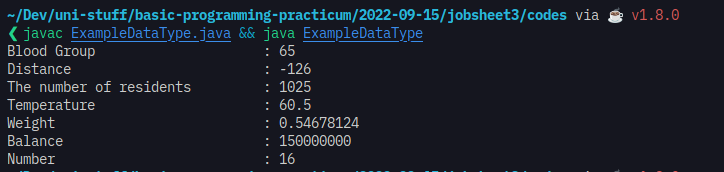
\includegraphics[width=0.9\textwidth]{./images/datatype-output.png}
            \caption{The output for Experiment 2}
        \end{figure}
    }
\end{enumerate}
\textbf{Questions}
\begin{enumerate}
    \item { 
        Explain why the \texttt{bloodGroup} does not display an "A"!

        Because we downcast the data type of \texttt{bloodGroup} from \texttt{char} (16bit) to a narrower type, which is \texttt{byte} (8bit).
    }
    \item {
        Explain the syntax of \texttt{byte distance = (byte) 130}! Then, explain why the results change when displayed!

        It's a syntax for casting to another data type. In this case, we're trying to downcast the number 130 to a \texttt{byte}.
        A byte can only contain -127 to 128, because of that there is integer overflow happening. Which explains why the number became -126 when it is displayed.
        We have 130, after it reaches 128 we still have 2 left, so it goes back to -127 and then continues to -126.
    }
    \item {
        In the syntax \texttt{float temperature = 60.50F}, remove the letter \texttt{F}, then run again. What happened?

        There will be a warning saying that there could possibly be a lossy conversion from \texttt{double} to \texttt{float}.
    }
    \item {
        Why does the result change when displaying \texttt{weight} values?

        Because we downcast it to \texttt{float}, we lost some precisions. \texttt{float} only stores 32bit of number while double can store up to 64bit, which explains why we lost some numbers after the comma.
    }
    \item {
        Explain the meaning of initializing \texttt{0x10} on \texttt{number} variables! What does it do?

        It is used to initialise a hexadecimal number, but because we initialise it as \texttt{int}, it is automatically converted.
        \texttt{0x10} in hexadecimal system is equal to 16 in decimal system.
    }
\end{enumerate}

\subsection{Experiment 3}
\begin{enumerate}
    \item Open a text editor
    \item Create a new file, give it a name \texttt{\textbf{ExampleOperator.java}}
    \item Write the basic structure of the Java programming language which contains the \texttt{main()} function.
    \item {
        Write the code below inside the \texttt{public static void main(String[] args)}

        \begin{figure}[h]
            \centering
            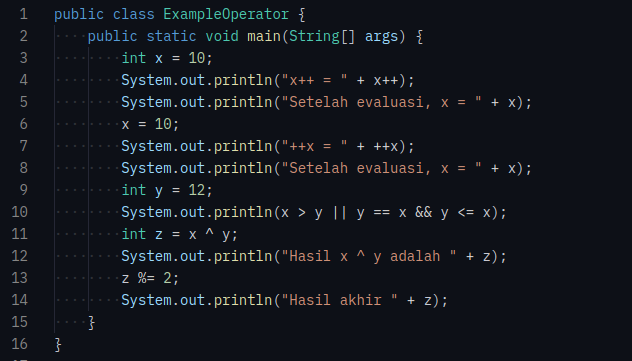
\includegraphics[width=0.9\textwidth]{./images/operator-code.png}
            \caption{The code for Experiment 3}
        \end{figure}
    }
    \item {
        Execute the program and observe the result

        \begin{figure}[h]
            \centering
            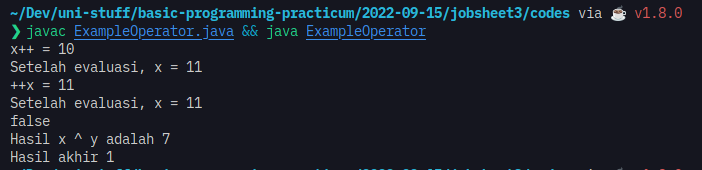
\includegraphics[width=0.9\textwidth]{./images/operator-output.png}
            \caption{The output for Experiment 3}
        \end{figure}
    }
\end{enumerate}
\pagebreak
\textbf{Questions}
\begin{enumerate}
    \item { 
        Explain according to your opinion what is the difference between \texttt{x++} and \texttt{++x}!

        What happens in \texttt{x++}, called post-increment, it assigns or use the current value and then increment it after it being used.
        While in \texttt{++x}, called pre-increment, it increments the value and then assign or use the current value.
        The difference between those two is the order of the incrementing process.
    }
    \item {
        What is the result of \texttt{int z = x \^{} y;} do the calculations manually (you can use a calculator)!

        It is a bitwise XOR operator. To calculate it manually, we first need to convert the decimal number into its binary equivalent. 
        Let $x = 11$ and $y = 12$.
        \begin{align*}
            x &= 11 / 2~(remainder~is~1)\\
              &= 5 / 2 ~(remainder~is~1)\\
              &= 2 / 2 ~(remainder~is~0)\\
              &= 1 / 2 ~(remainder~is~1)\\
            x &= 1011b\\~\\
            y &= 12 / 2~(remainder~is~0)\\
              &= 6 / 2 ~(remainder~is~0)\\
              &= 3 / 2 ~(remainder~is~1)\\
              &= 1 / 2 ~(remainder~is~1)\\
            y &= 1100b
        \end{align*}
        
        We can then apply the XOR as shown on this table. XOR returns \texttt{true} if one of the value is different, otherwise it will return \texttt{false}
        \begin{longtabu} to \textwidth {|c|c|c|}
            \caption{XOR Operation}\\
    
            \hline \multicolumn{1}{|c|}{\textbf{x}} & \multicolumn{1}{c|}{\textbf{y}} & \multicolumn{1}{c|}{\textbf{Output}} \\ \hline 
            \endfirsthead

            1 & 1 & 0\\
            0 & 1 & 1\\
            1 & 0 & 1\\
            1 & 0 & 1\\

            \hline
        \end{longtabu}
        The final result is \texttt{0111b}, in decimal system it is 7.
    }
\end{enumerate}

\pagebreak
\subsection{Experiment 4}

\begin{enumerate}
    \item Create a new file named \texttt{\textbf{Triangle.java}}
    \item {
        Observe the flowchart to calculate the area of the following triangle

        \begin{center}
            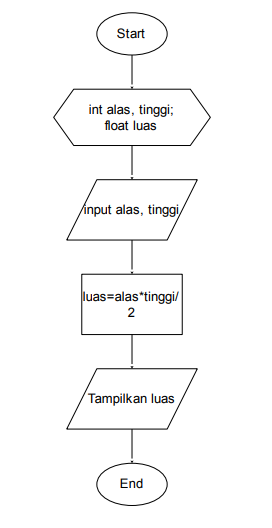
\includegraphics[width=6cm]{./images/flowchart.png}
        \end{center}
    }
    \item Create a basic Java program structure that consists of the \texttt{main()} function.
    \item {
        Add the \texttt{Scanner} library. Write the following code at the top outside the class
        \begin{minted}[autogobble, bgcolor=bg, fontsize=\scriptsize]{java}
            import java.util.Scanner;
        \end{minted}
    }
    \item {
        Make a \texttt{Scanner} declaration. Write the following code in the \texttt{main()} function
        \begin{minted}[autogobble, bgcolor=bg, fontsize=\footnotesize]{java}
            Scanner sc = new Scanner(System.in);
        \end{minted}
    }
    \pagebreak
    \item {
        Create an \texttt{int} variable for base and height, then a float variable for area.
        \begin{minted}[autogobble, bgcolor=bg, fontsize=\footnotesize]{java}
            int base, height;
            float area;
        \end{minted}
    }
    \item {
        Write down the syntax for inputting the \texttt{base} and \texttt{height} values
        \begin{minted}[autogobble, bgcolor=bg, fontsize=\footnotesize]{java}
            System.out.print("Insert the base: ");
            base = sc.nextInt();
            System.out.print("Insert the height: ");
            height = sc.nextInt();
        \end{minted}
    }
    \item {
        Write down the syntax for calculating the \texttt{area} of a triangle
        \begin{minted}[autogobble, bgcolor=bg, fontsize=\footnotesize]{java}
            area = base * height / 2
        \end{minted}
    }
    \item {
        Print the calculation of the \texttt{area} of the triangle
        \begin{minted}[autogobble, bgcolor=bg, fontsize=\footnotesize]{java}
            System.out.println("Triangle area: " + area);
        \end{minted}
    }
    \item Compile and run the program. Observe the results!
    \begin{figure}[h]
        \centering
        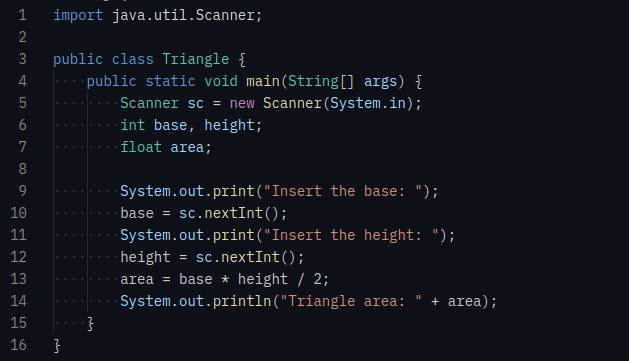
\includegraphics[width=0.9\textwidth]{./images/triangle-code.png}
        \caption{The code for Experiment 4}
    \end{figure}
    \begin{figure}[h]
        \centering
        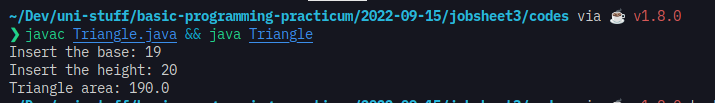
\includegraphics[width=0.9\textwidth]{./images/triangle-output.png}
        \caption{The result of Experiment 4}
    \end{figure}
\end{enumerate}
\pagebreak
\textbf{Questions}
\begin{enumerate}
    \item {
        Explain why the float data type is used for the variable area!

        Because we need its precision after doing arithmetic operation involving multiplication or division.
        If we use integer, the number will get rounded and we will lose some precision.
    }
\end{enumerate}

\end{document}

